
\documentclass[11pt]{article}
\usepackage{acl2014}
\usepackage{times}
\usepackage{url}
\usepackage{latexsym}
\usepackage{graphicx}
\usepackage{amsmath}

%\setlength\titlebox{5cm}

% You can expand the titlebox if you need extra space
% to show all the authors. Please do not make the titlebox
% smaller than 5cm (the original size); we will check this
% in the camera-ready version and ask you to change it back.


\title{Gesture Recognition with Recurrent Neural Networks}

\author{Justin Fu \\
  University of California, Berkeley\\
  {\tt justinfu@berkeley.edu} \\\And
  Siddhartho Bhattacharya \\
  University of California, Berkeley\\
  {\tt siddartho\_b@hotmail.com} \\}

\date{}

\begin{document}
\maketitle 
\begin{abstract}
  Gesture recognition is typically done through images, but it requires
  extensive effort to process image data into a form useful for gesture
  recognition. Our project uses accelerometer data from smartphones,
  so no special hardware is required.
  Recurrent neural networks provide a natural way to model time
  sequences, and the LSTM architecture in particular provides a way
  to model long-range dependencies that are prevalent in
  the gestures we tested. We imlemented X gestures, and achieve an
  accuracy of X percent on the test set we generated.
\end{abstract}

\section{Introduction}

Intro goes here.

\section{Data}

We collected accelerometer data streamed from a smartphone.

\section{Model}
\label{sect:pdf}

We implemented an LSTM (long short term memory) network based on
the architectures proposed by Graves [1]. Specifically,
our network contains the forget, input, and output gates, but lacks the
peephole connections that connect the internal cell state to these gates
(as done in Vinyals et al. [2]).

\begin{figure}[ht]
\caption{A single LSTM cell.}
  \centering
    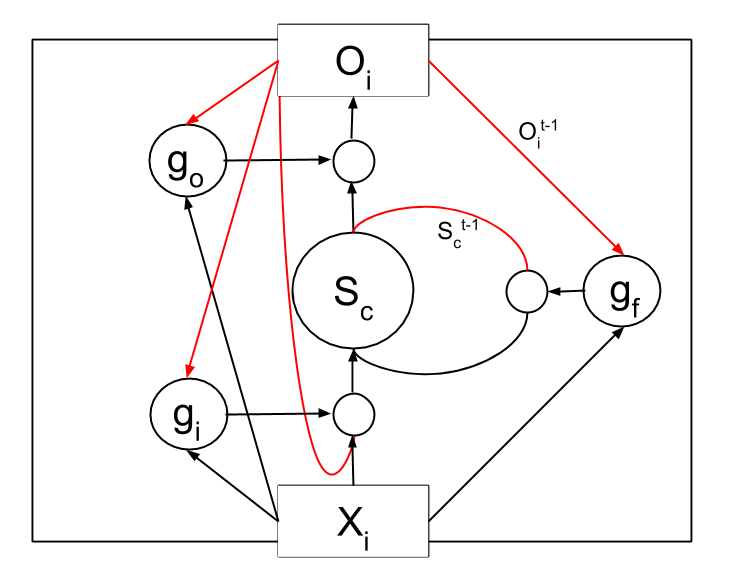
\includegraphics[width=0.5\textwidth]{lstm_cell}
\end{figure}

We then interleave layers of LSTM units with
normal network layers to create a multilayer network.

\subsection{Equations}

We used squared error as our objective function. \(O\) is the network
output and \(Y\) is the teacher value. \(n\) sums over each
training example, \(t\) sums over time, and \(i\) sums over the dimensions
of each training example at a given timestep.
Note that \(t\) varies with each training example.

\[  L(Y, O) = \sum_{n}^{N}  \sum_{t}^{len(O^{n})} \sum_{i}^{I} \frac{1}{2} (o_{i}^{n,t} - y_{i}^{n,t})^{2} \]

Most of the equations on the forward and backward passes are the
same as those in Graves [1], but some were missing so we specify all
for completeness.

\subsection{Forward Dynamics}
The forward dynamics of the network are specified as follows. Equations
are specified for a whole layer (rather than per unit).
 Bolded values represent vectors. Note that \(*\)
represents a point-wise multiply.

Gates
\[ \textbf{a}_{i} = W_{i,x}\textbf{x}^{t} +  W_{i,o}\textbf{o}^{t-1} \] 
\[ \textbf{g}_{i} = \sigma( \textbf{a}_{i}) \]
\[ \textbf{a}_{f} = W_{f,x}\textbf{x}^{t} +  W_{f,o}\textbf{o}^{t-1} \] 
\[ \textbf{g}_{f} = \sigma( \textbf{a}_{f}) \]
\[ \textbf{a}_{o} = W_{o,x}\textbf{x}^{t} +  W_{o,o}\textbf{o}^{t-1} \] 
\[ \textbf{g}_{o} = \sigma( \textbf{a}_{o}) \]

Cell State
\[ \textbf{a}_{c} = W_{c,x}\textbf{x}^{t} +  W_{c,o}\textbf{o}^{t-1} \] 
\[ \textbf{s}_{c} =  \textbf{g}_{i} * \sigma( \textbf{a}_{c}) + \textbf{g}_{f}*\textbf{s}_{c}^{t-1} \]

Cell Output (Hidden State)
\[ \textbf{o} =  \textbf{g}_{i} * \tanh( \textbf{s}_{c}) \]

Normal Layer Output
\[ \textbf{a}_{n} = W_{n}\textbf{o} \]
\[ \textbf{n} = \sigma( \textbf{a}_{n}) \]

\subsection{Backpropagation}
\(\delta_{k}^{L+1}\) represents the error backpropogating from the above layer. 
As with before, \(*\) represents a pointwise multiplication.

Cell Output
\[  \delta_{n} = \delta_{k}^{L+1}*\tanh'({\textbf{a}_{n}}) \]
\[ \delta_{h} = W_{i,h}^{T}\delta_{i}^{t+1} +  W_{f,h}^{T}\delta_{f}^{t+1} +  W_{o,h}^{T}\delta_{o}^{t+1} +  W_{c,h}^{T}\delta_{s}^{t+1} \]
\[ \frac{\partial L}{\partial \textbf{o}} = W_{n}^{T} \delta_{n} +  \delta_{h} \]

Gates
\[ \delta_{o} = \sigma'(\textbf{a}_{o}) * \tanh( \textbf{s}_{c}) *  \frac{\partial L}{\partial \textbf{o}} \]

BLAH

\section{Training}

We trained our network using BPTT (backpropogation through time) and
gradient descent with momentum.

\section{Decoding}

\section{Example \LaTeX stuff}
\begin{itemize}
\item Item  Example 1
\item Item Example 2
\end{itemize}

\begin{table}[h]
\begin{center}
\begin{tabular}{|l|rl|}
\hline \bf Column & \bf Col & \bf Col \\ \hline
row blah & blah & blah \\
row blah & blah & blah \\
\hline
\end{tabular}
\end{center}
\caption{\label{font-table} Example table! }
\end{table}

\noindent Noindent


\subsection{subsection}

\begin{quote}
\begin{verbatim}
\usepackage{times}
\usepackage{latexsym}
\end{verbatim}
\end{quote}

\begin{quote}
  ``\cite{Graves:08} Quote''
\end{quote}

\subsection{Sections}

{\bf Citations}: Citations within the text appear in parentheses
as~\cite{Gusfield:97} or, if the author's name appears in the text
itself, as Gusfield~\shortcite{Gusfield:97}.  Append lowercase letters
to the year in cases of ambiguity.  Treat double authors as
in~\cite{Aho:72}, but write as in~\cite{Chandra:81} when more than two
authors are involved. Collapse multiple citations as
in~\cite{Gusfield:97,Aho:72}. Also refrain from using full citations
as sentence constituents. We suggest that instead of

you use
\begin{quote}
``Gusfield \shortcite{Gusfield:97}   showed that ...''
\end{quote}

If you are using the provided \LaTeX{} and Bib\TeX{} style files, you
can use the command \verb|\newcite| to get ``author (year)'' citations.

As reviewing will be double-blind, the submitted version of the papers
should not include the authors' names and affiliations. Furthermore,
self-references that reveal the author's identity, e.g.,
\begin{quote}
``We previously showed \cite{Gusfield:97} ...''  
\end{quote}
should be avoided. Instead, use citations such as 
\begin{quote}
``Gusfield \shortcite{Gusfield:97}
previously showed ... ''
\end{quote}

\subsection{Footnotes}

{\bf Footnotes}: Put footnotes at the bottom of the page and use 9
points text. They may be numbered or referred to by asterisks or other
symbols.\footnote{This is how a footnote should appear.} Footnotes
should be separated from the text by a line.\footnote{Note the line
separating the footnotes from the text.}


\section*{Acknowledgments}

Brian is our savior.

% include your own bib file like this:
%\bibliographystyle{acl}
%\bibliography{acl2014}

\begin{thebibliography}{}

\bibitem[\protect\citename{Graves}2008]{Graves:08}
[1]
Alex Graves.
\newblock 2008.
\newblock {\em Supervised Sequence Labelling with Recurrent Neural Networks}.
\newblock PhD Thesis.

\bibitem[\protect\citename{Vinyals}2014]{Vinyals:14}
[2]
Orial Vinyals, Alexander Toshev, Samy Bengio, Dumitru Erhan.
\newblock 2014.
\newblock {\em Show and Tell: A Neural Image Caption Generator}.

\end{thebibliography}

\end{document}
